\documentclass[compress,12pt]{beamer}
\nocite{*}

\addtobeamertemplate{navigation symbols}{}{%
    \usebeamerfont{footline}%
    \usebeamercolor[fg]{footline}%
    \hspace{1em}%
    \insertframenumber/\inserttotalframenumber
}

\usetheme{Arguelles}

\title{Multiagent Reinforcement Learning for Traffic Signal Control}
\event{}
\date{March 20, 2024}
\author{Kevyn Kelso}
\institute{University of Colorado at Colorado Springs}
\email{kkelso@uccs.edu}
\github{KevynKelso}

\begin{document}

\frame[plain]{\titlepage}

\Section{Introduction}

\begin{frame}[bg=arguelles.png]
      \frametitle{Table of Contents}
      \begin{itemize}
      \item Review: MDP Problem and Existing Methods
      \item Experimental Methodology
      \item Results
      \item Challenges Faced
      \item Remaining Timeline
      \end{itemize}
\end{frame}

\Section{Review}

\begin{frame}[bg=arguelles.png]
      \frametitle{Review - MDP State Space}
      \begin{itemize}
      \item Signalized intersections contribute to 12-55\% of commute time, with RL methods potentially reducing this by 73\%, guiding this project's aim to enhance RL traffic control strategies.
      \item TSC as a POMDP involves partial state visibility and non-stationary dynamics, leading to state aliasing and challenges in centralized approaches due to dimensionality and infrastructure demands.
      \item State Space modeled in \ref{eq:state_space}. \(\rho\) are intersection state variables, \(\Delta_l\) are lane density variables, and \(l \in L\) is No. queued vehicles for each lane.
      \end{itemize}

\begin{equation}
s_t = [\rho_1, \rho_2, g, \Delta_1, \ldots, \Delta_L, q_1, \ldots, q_L]
\label{eq:state_space}
\end{equation}
\end{frame}


\begin{frame}[bg=arguelles.png]
      \frametitle{Review - MDP Action Space}
      \begin{itemize}
      \item Agent can select an action to put the intersection into one of four modes \(a_t \in \{a_1, a_2, a_3, a_4\}\).
      \item To change the intersection into a different mode, a mandatory yellow phase $\phi$ precedes the mode change.
      \end{itemize}

    \begin{figure}[htbp]
      \centering
      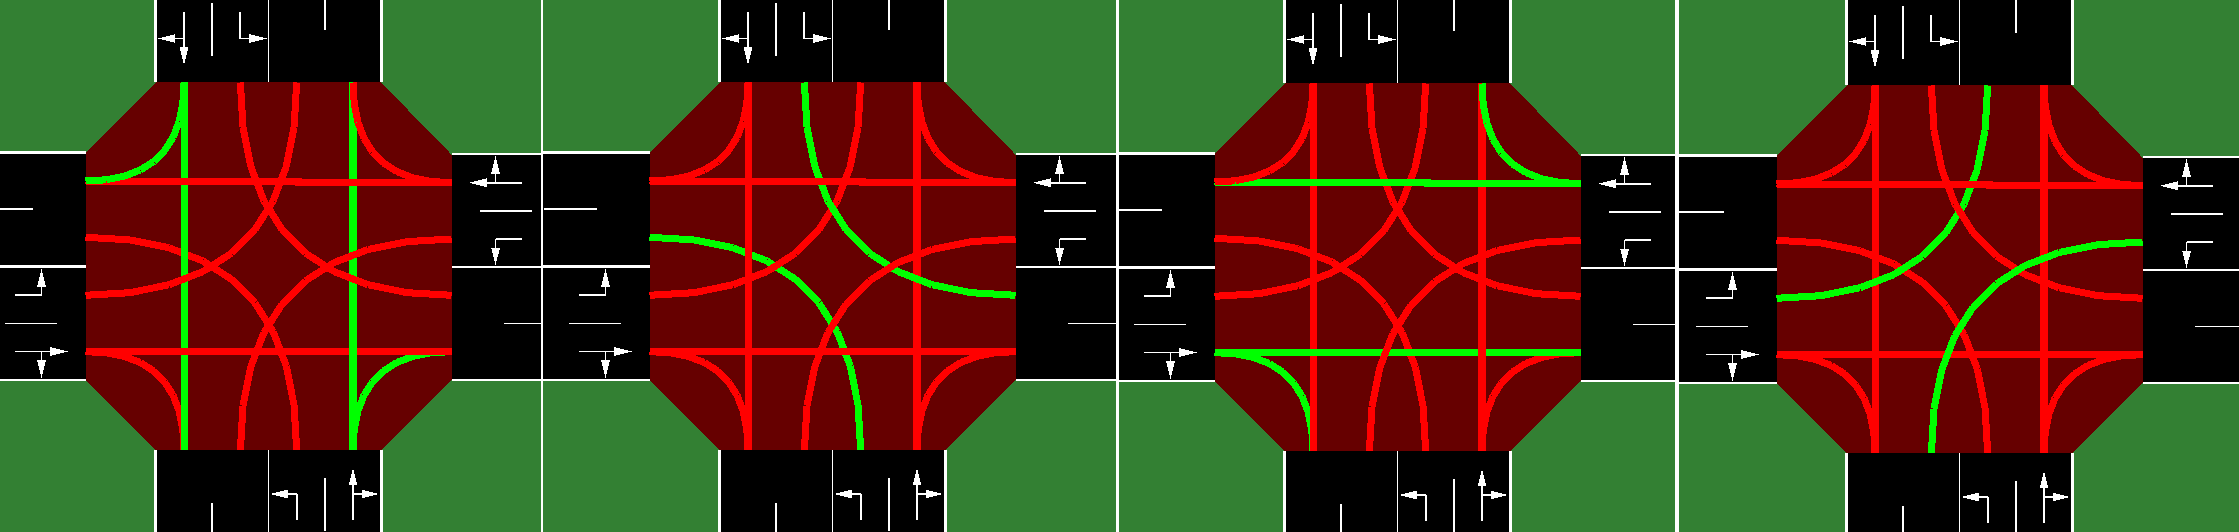
\includegraphics[width=0.8\linewidth]{actions.png}
      \caption{Traffic light modes}
      \label{fig:action_space}
    \end{figure}
\end{frame}

\begin{frame}[bg=arguelles.png]
      \frametitle{Review - Analyzing Cumulative Delay in MDP Framework}
      \begin{itemize}
        \item Reward function cumulative delay $D_t$ is defined, summing all vehicle wait times at time $t$ (\ref{eq:cumulative_delay}) to compute immediate rewards $r_t$.
        \item The same reward signal is applied to all agents in the system encouraging cooperation.
        \item $r_t$ represents the reward at time $t$, calculated by the reduction in cumulative delay $D_t$ where $d_t^v$ is the wait time of vehicle $v$ at time $t$.
      \end{itemize}

    \begin{equation}
    r_t = D_t - D_{t+1}
    \label{eq:cumulative_delay}
    \end{equation}

    \begin{equation}
    D_t = \sum_{v \in V_t} d_t^v
    \label{eq:wait_time_sum}
    \end{equation}
\end{frame}

\Section{Methods}

\begin{frame}[bg=arguelles.png]
      \frametitle{Review - Existing Methods}

    \begin{table}[H]
    \centering
    \small
    \begin{tabular}{lc}
    \hline
    \textbf{Method} & \textbf{Average Cumulative Delay (seconds)} \\ \hline
    \textbf{Fixed Time}      & \textbf{90.00}\footnotemark[2]  \\
    Max Pressure    & 70.00\footnotemark[2]  \\
    Greedy          & 60.00\footnotemark[2]  \\
    \textbf{IDQN}            & \textbf{30.74}                  \\
    IPPO            & 36.15                  \\
    MPLight         & 54.58                  \\
    MA2C            & 38.07\footnotemark[1]                  \\
    FMA2C           & 42.26                  \\
    \(SARSA(\lambda)\)           & 18.00\footnotemark[2]                  \\
    Ontology        & 17.00\footnotemark[2]                  \\ \hline
    \end{tabular}
    \caption{Average Delay Across All Scenarios}
    \label{tab:avg_delay}
    \end{table}
    \footnotetext[1]{Data was only collected in one scenario and may not reflect how the model performs in other scenarios.}
    \footnotetext[2]{Data was extracted from graphs.}
\end{frame}

\begin{frame}[bg=arguelles.png]
      \frametitle{Experimental Methodology - IDQN}
      \begin{itemize}
        \item IDQN for traffic signal control: an off-policy, model-free RL approach.
        \item A deep neural network is used to approximate Q-values, predicting rewards for actions in given states.
        \item Experience is gained through interaction, employing shuffled training to refine network predictions. Replay buffer size = 100,000
        \item Dual-network architecture (target and trainer) for stable updates.
        \item $\epsilon$-greedy policy for action selection.
        \item Each traffic signal is independently managed by an IDQN.
      \end{itemize}
\end{frame}

\begin{frame}[bg=arguelles.png]
      \frametitle{Experimental Methodology - Convolutional IDQN}
      \begin{itemize}
        \item Switched from fully connected to a convolutional network for enhanced spatial feature capture in state representation.
        \item The state can be represented as an image where a 2x2 kernel convolves grouping state information to improve decision-making accuracy.
      \end{itemize}

      \begin{figure}[htbp]
        \centering
        \includegraphics[width=0.8\linewidth]{state_image_rep.png}
        \caption{Example of Image-Based State Representation in Convolutional IDQN}
        \label{fig:state_image_rep}
      \end{figure}
\end{frame}
\begin{frame}[bg=arguelles.png]
      \frametitle{Experimental Methodology - Convolutional IDQN}
      \begin{itemize}
        \item Table \ref{tab:model_summary} summarizes the convolutional model architecture. The original fully connected model contained a Dense + LeakyReLU on the first layer.
        \item This method yields a 20-second improvement in cumulative delay on the 4x4 grid over the fully connected architecture.
      \end{itemize}

      \begin{table}[h]
      \centering
      \begin{tabular}{lc}
      \hline
      \textbf{Layer (type)}              & \textbf{Param \#} \\ \hline
      \texttt{Conv2D + LeakyReLU}        & 320       \\
      \texttt{Flatten}                   & 0         \\
      \texttt{Dense + LeakyReLU}         & 81,984    \\
      \texttt{Dense + LeakyReLU}         & 4,160     \\
      \texttt{Dense}                     & 260       \\ \hline
      \textbf{Total trainable params}    & 86,724    \\ \hline
      \end{tabular}
      \caption{Q-Network Model Summary}
      \label{tab:model_summary}
      \end{table}

\end{frame}

\begin{frame}[bg=arguelles.png]
      \frametitle{Experimental Methodology - Huber Loss}
      \begin{itemize}
        \item Huber loss (\ref{eq:huber_loss}) combines the best of Mean Squared Error (MSE) and absolute loss, offering outlier resistance, and enhancing Q-network training. Better performance was seen over MSE and cross-entropy.
        \item Combines $L_{abs}(x) = |x|$ and $L_{quadratic}(x) = x^2$.
        \item Smoothly transitions from quadratic to linear (at $\delta=1.0$), optimizing learning.
      \end{itemize}

\begin{equation}
   \label{eq:huber_loss}
    L_{\delta}(x) = \left\{ 
    \begin{array}{ll}
      \frac{1}{2}x^{2}, & \text{for } |x| \leq \delta \\
      \delta\left(|x| - \frac{1}{2}\delta\right), & \text{for } |x| > \delta
    \end{array}
    \right.
\end{equation}
\end{frame}

\section{Results}

\begin{frame}[bg=arguelles.png]
  \frametitle{Fixed Time Baseline Results - Single Intersection}
  \begin{itemize}
    \item Fixed time agent implemented with a round-robin approach, cycling every 50 seconds.
    \item Average cumulative delay from fixed time algorithm: 90 seconds across various scenarios. 45 seconds single intersection.
  \end{itemize}
  \begin{figure}
    \centering
    \includegraphics[width=0.6\linewidth]{delays_fixed_single.png}
    \caption{Avg. Delay RR Single Signal}
  \end{figure}
\end{frame}

\begin{frame}[bg=arguelles.png]
  \frametitle{Convolutional DQN Results - Single Intersection}
  \begin{itemize}
    \item Convolutional DQN applied to a single intersection, assessing average cumulative delay and Huber loss.
  \end{itemize}
  \begin{minipage}{.5\textwidth}
    \centering
    \includegraphics[width=\linewidth]{delays_dqn_single.png}
  \end{minipage}%
  \begin{minipage}{.5\textwidth}
    \centering
    \includegraphics[width=\linewidth]{loss_dqn_single.png}
  \end{minipage}
\end{frame}

\begin{frame}[bg=arguelles.png]
  \frametitle{Convolutional IDQN Results - 4x4 Grid}
  \begin{itemize}
    \item Overview of fixed time results for 4x4 grid: Average 60 seconds delay, ~100 stopped vehicles.
    \item Introduction of 16 convolutional IDQN agents for traffic signal control.
  \end{itemize}
  \begin{minipage}{.5\textwidth}
    \centering
    \includegraphics[width=\linewidth]{../sumo-rl/Data_dqn_multi_2/avg_delay.png}
  \end{minipage}%
  \begin{minipage}{.5\textwidth}
    \centering
    \includegraphics[width=\linewidth]{../sumo-rl/Data_dqn_multi_2/total_stopped.png}
  \end{minipage}
\end{frame}

\begin{frame}[bg=arguelles.png]
  \frametitle{Huber Loss - 4x4 Grid DQN Agents}
  \begin{figure}
    \centering
    \includegraphics[width=0.9\linewidth]{../sumo-rl/Data_dqn_multi_2/dqn_trainer_loss.png}
  \end{figure}
\end{frame}


\Section{Conclusion}
\begin{frame}[bg=arguelles.png]
      \frametitle{Challenges Faced}
      \begin{itemize}
      \item Non-stationary dynamics in multiagent 4x4 grid increase complexity compared to single-agent environments.
      \item Fully connected IDQN agents underperformed in the 4x4 grid, leading to the exclusive use of convolutional IDQN agents.
      \item Utilized research projects for project bootstrap \footnote{https://github.com/LucasAlegre/sumo-rl} \footnote{https://github.com/jault/StateStreetSumo}, requiring debugging and extension for TensorFlow 2.x compatibility, and additional feature integration.
      \end{itemize}
\end{frame}

\begin{frame}[bg=arguelles.png]
      \frametitle{Timeline}

\begin{table}[H]
\centering
\begin{tabular}{lll}
\hline
\textbf{Done} & \textbf{Date} & \textbf{Milestone}             \\ \hline
\checkmark & 2/19 & 4x4 grid environment setup and working  \\
\checkmark & 2/26 & IDQN agents learning                    \\
\checkmark & 3/4  & Perform experiments and generate data   \\
& 3/18 & Injected uncertainty scenarios          \\
& 3/24 & Binary DQN experiments                  \\
& 4/1 & Double DQN and other misc experiments  \\
& 4/15 & Data compilation and writing            \\
& 4/20 & Simulate Colorado Springs? \\ \hline
\end{tabular}
\caption{Project Timeline}
\label{tab:project_timeline}
\end{table}
\end{frame}

\begin{frame}[allowframebreaks]
        \frametitle{References}
        \bibliographystyle{amsalpha}
        \bibliography{proposal.bib}
\end{frame}

\begin{frame}[plain,standout]
      \centering
      Any questions? \\
      \vfill
    \begin{figure}[htbp]
      \centering
      \includegraphics[width=0.7\linewidth]{wpid-images-7.png}
    \end{figure}
\end{frame}

\end{document}
